\subsection{Package \lstinline!cryptocast.client.filechooser!}
A generic implementation of a file chooser for Android applications.

\noindent\begin{minipage}[t]{5cm}
\vspace{0.3em}
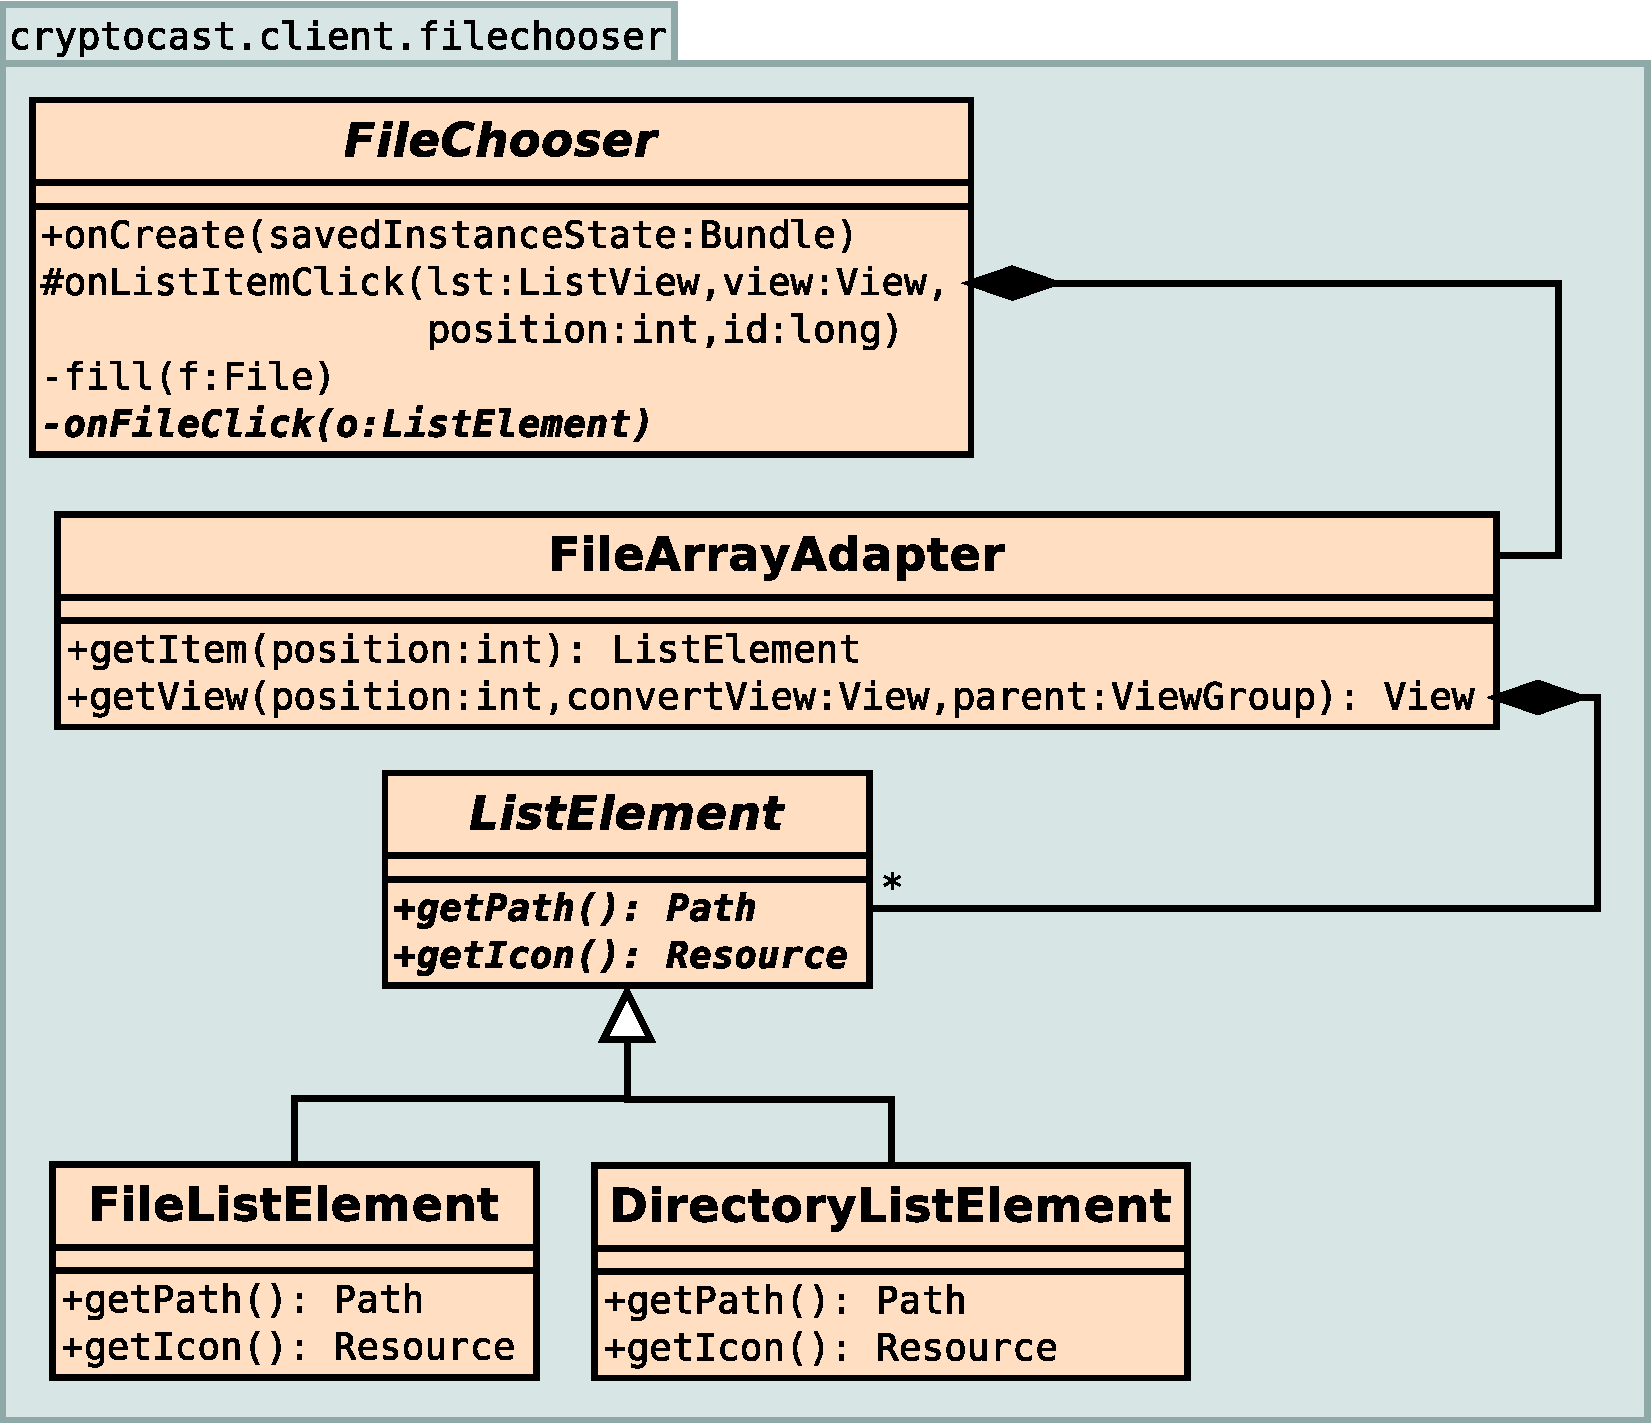
\includegraphics[width=300px]{class_diagrams/cryptocast_client_filechooser.pdf}
\end{minipage}

\subsubsection{Class \lstinline|FileListElement|}
A list element in our file chooser, representing a file. \\
\noindent\begin{minipage}[t]{5cm}
\vspace{0.3em}
\hspace*{2em}
\begin{tikzpicture}
\umlclass[]{FileListElement}{

}{
+ getPath() : Path \\ + getIcon() : Resource
}
\end{tikzpicture}
\vspace{0.3em}
\end{minipage}



\textbf{\sffamily Superclasses and Interfaces}
\begin{itemize}
\item \lstinline|cryptocast.client.filechooser.ListElement|
\end{itemize}


\textbf{\sffamily Constructors}
\begin{itemize}
\item \lstinline|public| \lstinline|FileListElement|\lstinline|(Path path)|\\ \\[-0.6em]
Creates a new instance.
\begin{itemize}
\item \lstinline|path|: The path of the file
\end{itemize}



\end{itemize}


\textbf{\sffamily Methods}
\begin{itemize}
\item \lstinline|public Path| \lstinline|getPath|\lstinline|()|\\ \\[-0.6em]
\emph{Returns:} The path of the element



\item \lstinline|public Resource| \lstinline|getIcon|\lstinline|()|\\ \\[-0.6em]
\emph{Returns:} The icon associated with this element.



\end{itemize}

\subsubsection{Interface \lstinline|ListElement|}
A list element in our file chooser, representing an element on the file system. \\
\noindent\begin{minipage}[t]{5cm}
\vspace{0.3em}
\hspace*{2em}
\begin{tikzpicture}
\umlclass[type=abstract]{ListElement}{

}{
\umlvirt{+ getPath() : Path} \\ \umlvirt{+ getIcon() : Resource}
}
\end{tikzpicture}
\vspace{0.3em}
\end{minipage}





\textbf{\sffamily Methods}
\begin{itemize}
\item \lstinline|public Path| \lstinline|getPath|\lstinline|()|\\ \\[-0.6em]
\emph{Returns:} The path of the element



\item \lstinline|public Resource| \lstinline|getIcon|\lstinline|()|\\ \\[-0.6em]
\emph{Returns:} The icon associated with this element.



\end{itemize}


